\documentclass{article} % For LaTeX2e
\usepackage{nips15submit_e,times}
\usepackage{hyperref}
\usepackage{url}
\usepackage{graphicx}
\usepackage{amssymb}
%\documentstyle[nips14submit_09,times,art10]{article} % For LaTeX 2.09

\title{Using Recurrent Neural Networks on the WAY-EEG-GAL dataset}

\author{
Roman C.~Podolski
\\
%Technische Universit\"at M\"unchen\\
%Pittsburgh, PA 15213 \\
\texttt{roman.podolski@tum.de} \\
\And
Dominik Irimi \\
%Affiliation \\
%Address \\
\texttt{dominik.irimi@tum.de} \\
\AND
Christoph Dehner \\
%Affiliation \\
%Address \\
\texttt{dehner@in.tum.de} \\
\And
Manuel Nickel \\
%Affiliation \\
%Address \\
\texttt{manuel.nickel@tum.de} \\
\And
Philipp Bergmann \\
%Affiliation \\
%Address \\
\texttt{philipp.bergmann@tum.de} \\
}

% The \author macro works with any number of authors. There are two commands
% used to separate the names and addresses of multiple authors: \And and \AND.
%
% Using \And between authors leaves it to \LaTeX{} to determine where to break
% the lines. Using \AND forces a linebreak at that point. So, if \LaTeX{}
% puts 3 of 4 authors names on the first line, and the last on the second
% line, try using \AND instead of \And before the third author name.

\newcommand{\fix}{\marginpar{FIX}}
\newcommand{\new}{\marginpar{NEW}}

\nipsfinalcopy % Uncomment for camera-ready version

\begin{document}


\maketitle

\begin{abstract}
The \emph{WAY-EEG-GAL} dataset is designed to allow testing of techniques to decode sensation, intention and action from scalp EEG recordings in humans who perform a grasp-and-lift task. In this paper we present our methodology to analyze the data and how we tackled the problem of classifying various stages of these tasks by using a RNN on EEG and EMG data. In particular we present particular findings in the EEG data and successes as well as pitfalls concerning the RNN runs.
\end{abstract}

\section{About the WAY-EEG-GAL dataset}\label{sec:tsne}
In order to allow for critical evaluations of the utility of EEG signals for prosthetic control of object manipulation, the \emph{Wearable interfaces for hAnd function recoverY - EEG - Grisp And Lift (WAY-EEG-GAL)} dataset was created. In particular, it can be used to inter alia examine at what degree it is possible to identify the intention to reach and grasp, hand positions and velocities or that the object's properties have unexpectedly changed. The data was collected during the course of a series of experiments in which twelve right-handed individuals, both male and female, were selected as participants. Each participant was seated at a desk with his hand resting on the table. An LED signaled the person to reach for a small object, grasp it using his index finger and thumb, lift it up a few centimetres, hold it for a brief moment and finally return the object as well as his hand to their intial positions. In this paper, we will from now on refer to this sequence of events and actions as a \emph{trial}. \\
Each participant then conducted $328$ such trials under slight but to the participant unpredictably changing circumstances. That is, the object's weight to be lifted was augmented through an electromagnet, resulting in weights of $165$, $330$ or $660 g$. Furthermore, the contact surface changed to be made of sandpaper, suede or silk. Depending on the specific trial, either only the surface, only the object's weight, both or none changed. In order to record kinematics, forces, muscle activations and brain activity, four types of sensors were used during the experiments. In particular, an electroencephalography (EEG) cap, illustrated in figure \ref{fig:eeg_setup}, with $32$ electrodes was used to record the brain activity during the trials, sampling at $500 Hz$. Furthermore, five electromyography (EMG) sensors, as depicted in figure \ref{fig:emg_setup}, were placed on the participant's right arm to measure muscle activity at a sample rate of $4 kHz$.\\
\begin{figure}
	\centering
	\begin{minipage}{0.5\textwidth}
		\centering
		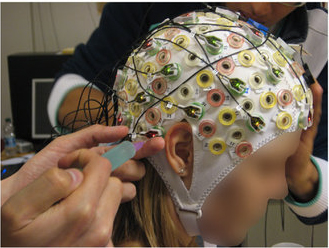
\includegraphics[width=1.0\textwidth]{images/eeg_setup.jpg}
		\caption{An EEG cap measures the participant's brain activity \cite{nature}}
		\label{fig:eeg_setup}
	\end{minipage}\hfill
	\begin{minipage}{0.49\textwidth}
		\centering
		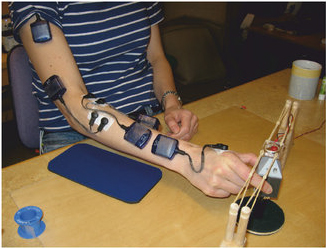
\includegraphics[width=1.0\textwidth]{images/emg_setup.jpg}
		\caption{EMG sensors record the muscle activity of the right arm \cite{nature}}
		\label{fig:emg_setup}
	\end{minipage}
\end{figure}
The resulting dataset, in the form that we used it, then provides the measurements for each participant and each trial. In this, the EEG and EMG signals are concatenated in matrices respectively with a time stamp decoding the exact record time for each measurement. Moreover, the time of the LED being turned on and off, the trial's start and end time, the type of surface and the object's weight are provided for each trial, as well. \cite{nature}




\section{Analyzing the datas using t-SNE}
In order to get a \emph{feeling} for how the EEG as well as EMG datasets are inherently structured, we aimed to visualize them. In particular, we were interested in how the notion of \emph{grasping an object} is captured. That is, does an individual measurement by itself carry enough information allowing to conclude that the participant is right now grasping an object or not? Or is this notion rather encapsulated within a series of measurements, with datapoints that change over time?\\
As the individual datapoints are high-dimensional ($\mathcal{D}_{EEG} \in \mathbb{N}^{32}$ and $\mathcal{D}_{EMG} \in \mathbb{R}^5$ respectively), a particularly suitable method of visualization seemed t-distributed stochastic neighbourhood embedding (t-SNE), which allows to represent high-dimensional data as a two-dimensional mapping by grouping similar state vectors close together and separating them from less similar ones. Specifically, we used an efficient Barnes Hut t-SNE implementation, created by L.J.P. van der Maaten [2]. Doing so, we created t-SNE plots of the EEG as well as the EMG data. An important property of t-SNE is that it cannot consider time-relations between individual data points, instead it sees each data point as its own entity. However, in order to make sure that the used implementation of t-SNE is not somehow influenced by the ordering of the states, all data points were shuffled and placed in random order before being fed to t-SNE.\\
In the following, we have a look at a subset of the WAY-EEG-GAL dataset. In particular we exemplarily examine participant $1$'s first series, a dataset composed of $34$ trials in total, which are collected in \verb|WS_P1_S1.mat|. Each of the 34 trials were marked with a different color in the resulting plot, e.g. states of trial $1$ might be colored in green while states of trial $2$ in red. Furthermore, states that were measured within the time span of the LED being lid up are drawn with a black border in order to separate them visually from states with the LED being off.\\
Doing so, we expected to see one of these possible outcomes:
\begin{itemize}
	\item The LEDon-states are grouped together in one place while the LEDoff-states are grouped in another place:
	We interpret this a sign that it is possible to extract information about the intention to grasp from individual data points. As t-SNE does not \emph{understand} relations in time, even a simple Feedforward Net might work.
	\item All data points are distributed randomly and there is no apparent structure in the plot:
	This would signal that if there is a way to extract information about the intention to grasp, then it is not sufficient to use Feedforward Nets only. Instead, one needs to at least incorporate time relations. Thus, we try using Recurrent Neural Nets.
\end{itemize}
Figure \ref{fig:emg_tsne} shows the t-SNE plot for the $34$ trials of participant $1$, series $1$. Clearly, all data points are distributed randomly and no particular grouping is to be seen. Following the reasoning described above, we conclude that using a Feedforward Neural Net cannot suffice to extract the grasping notion out of the EMG data.
\begin{figure}
	\centering
	\begin{minipage}{0.5\textwidth}
		\centering
		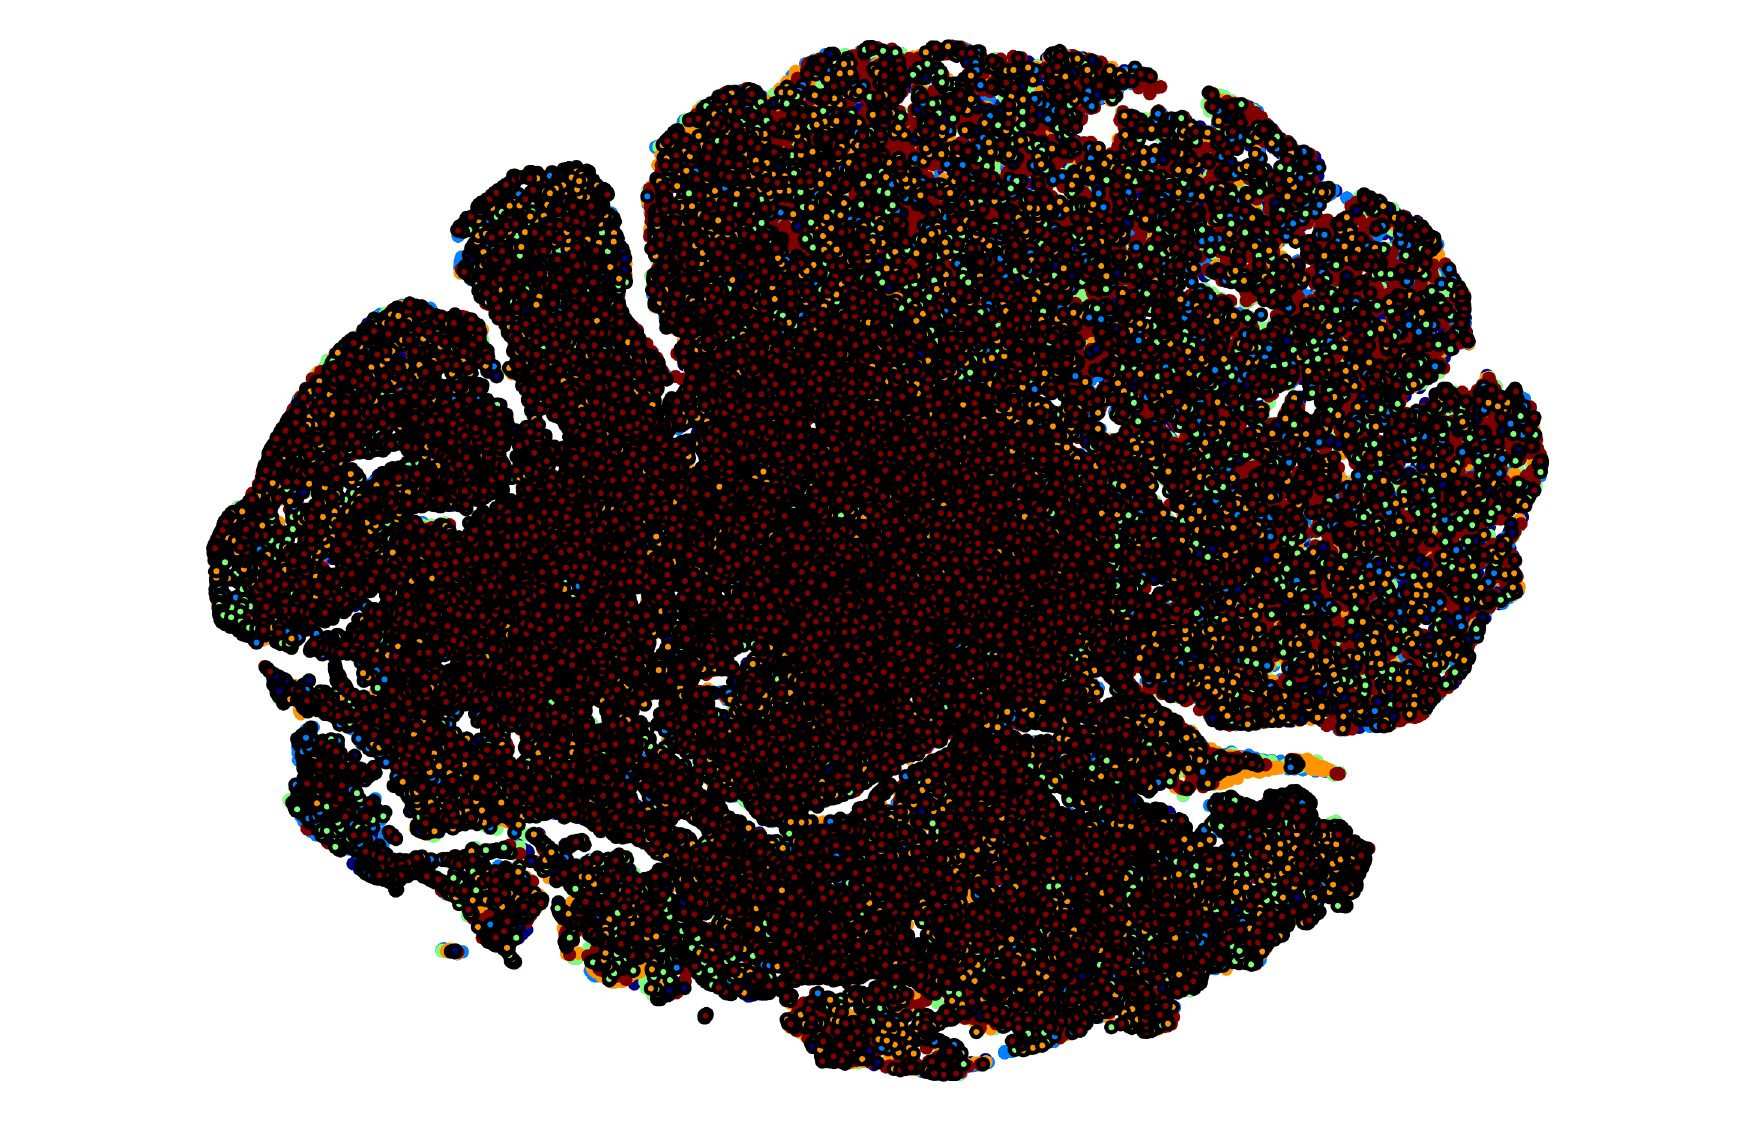
\includegraphics[width=1.0\textwidth]{images/emg_tsne.png}
		\caption{t-SNE plot for EMG data}
		\label{fig:emg_tsne}
	\end{minipage}\hfill
	\begin{minipage}{0.5\textwidth}
		\centering
		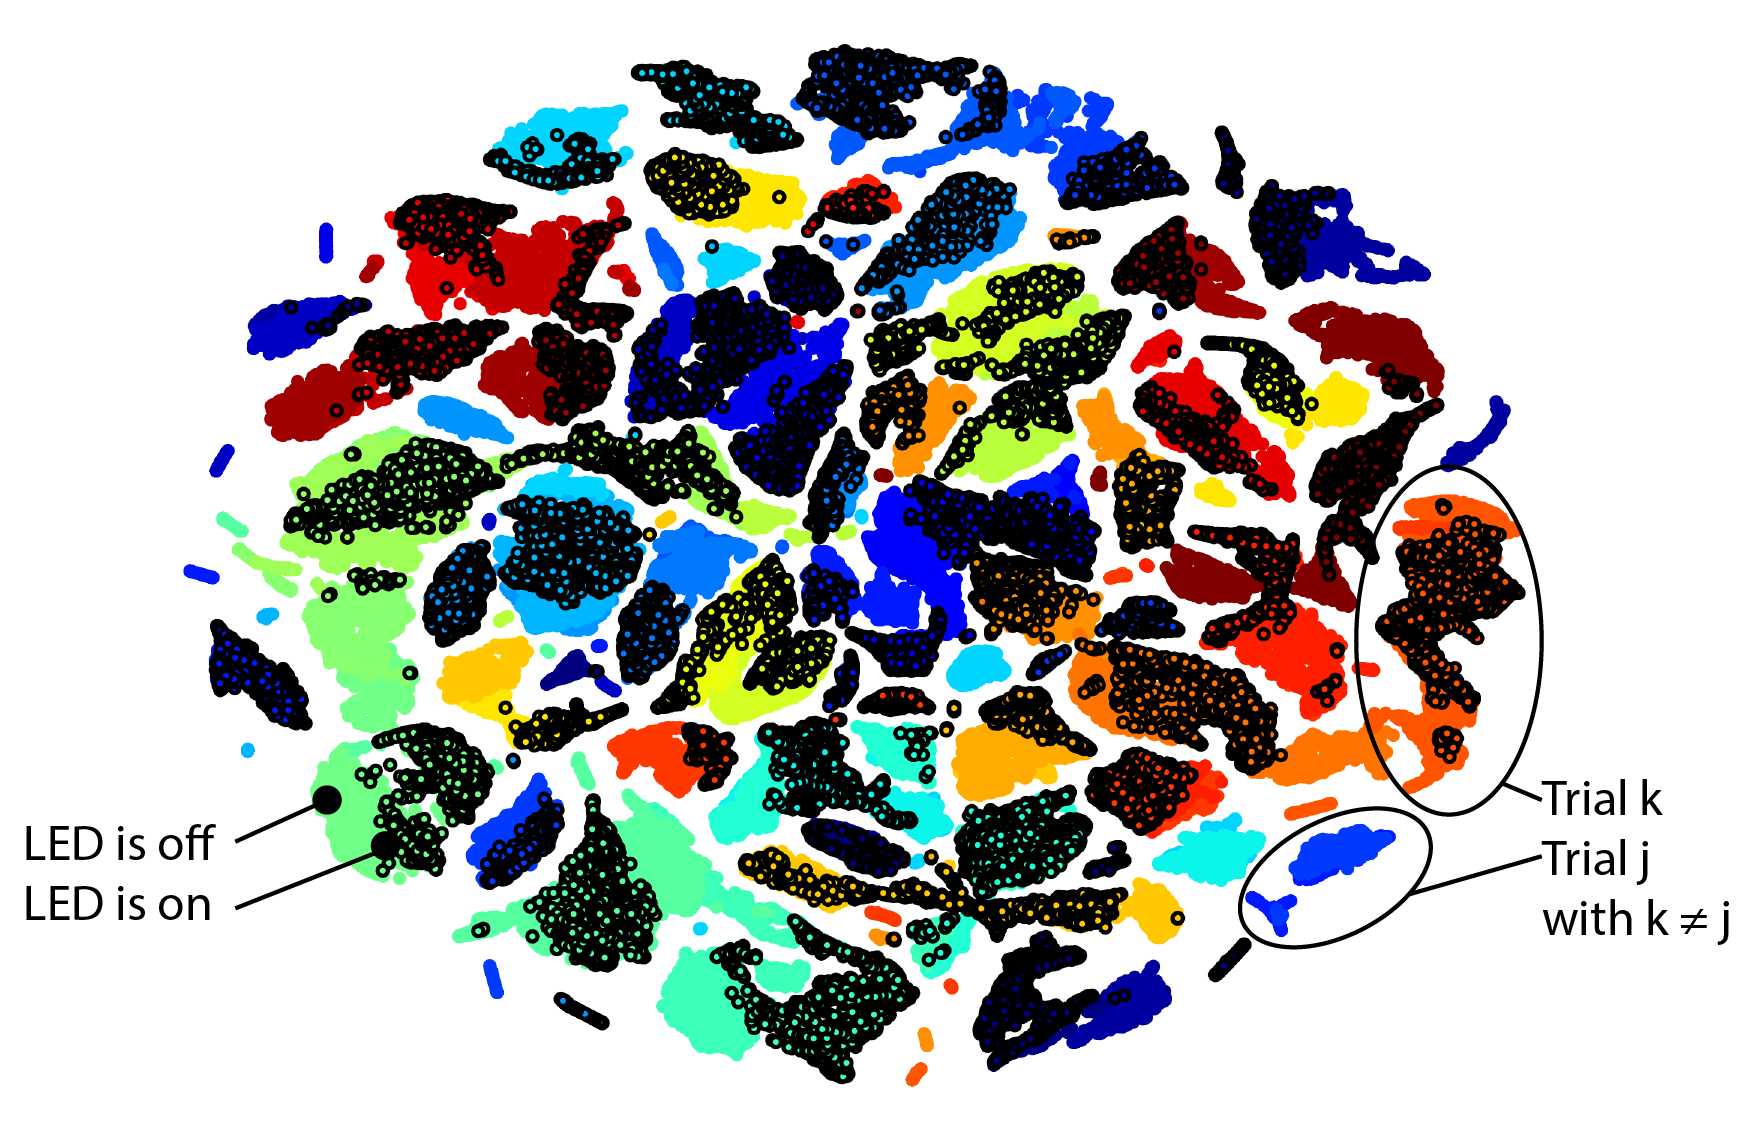
\includegraphics[width=1.0\textwidth]{images/eeg_tsne.png}
		\caption{t-SNE plot for EEG data}
		\label{fig:eeg_tsne}
	\end{minipage}
\end{figure}\\
We then applied the same t-SNE implementation to the EEG data. The result can be viewed in figure \ref{fig:eeg_tsne}. Here, the plot shows none of the expected characteristics. Instead, data points belonging to the same trial clearly form clusters while these clusters, each representing a specific trial, are then separated from each other. This indicates, that the EEG data somehow comprises a notion of time, encoding which measurement was taken during which trial. This is, however, not reasonable as the individual measurements are expected to be independent from each other. Thus, we first veryfied multiple times and using different methods the correct function of the t-SNE implementation, making sure the plots are no result of merely faulty computation. But, the implementation turned out to be working fine.\\
In this case, however, figure \ref{fig:eeg_tsne} suggests that it should be possible to determine for a given data point, i.e. measurement, during which trial it was taken. This comes down to a classification problem which can be solved using a simple Feedforward Neural Net.\\
Thus, we created a Neural Net with one hidden layer, $32$ input neurons and $300$ hidden neurons. Furthermore, a tanh activation function and gradient descent optimization were used. The EEG data from participant $1$, series $1$ contains $146982$ samples in $34$ trials, which were put in random order and partitioned into a training-, validation- and test-set containing $4/9$, $2/9$ and $1/9$ of the original samples respectively. The dataset was normalized to contain values between $-1$ and $+1$. In particular, each trial was normalized separately in order to remove a possible offset in the data, which might have caused the clustering in figure \ref{fig:eeg_tsne}.
However, the Neural Net confirmed the t-SNE results: Using above settings, a test error of only $2.38\%$ was achieved for participant $1$, series $1$. The Neural Net was applied to a variety of other subsets of WAY-EEG-GAL, too. There, even better test errors of just about $0.01\%$ were achieved. Overall, for any participant and series, the specific trials could be classified very easily by simply looking at a single measurement.\\
The above results suggest, that indeed information about the time of measurement is included within the measurements themselves. We suspect a continuous change in value for at least a subset of the electrodes measuring the brain activity, leading to characteristic patterns within each trial's data. We then applied various techniques trying to remove these unwanted characteristics. For this, different normalization and filtering methods with varying parameters were used. However, none of these succeeded. In fact, the normalization applied in above example even improved the Neural Net test error significantly: Without normalization a test error of comparatively bad $19.69\%$, with normalization a test error of $2.38\%$ was achieved.
Moreover, classification of trials turned out to be possible not only within a single series but over many more, too. For this, a Neural Net run was performed on the entire EEG data of participant $1$, comprising $294$ trials in total. This resulted in a test error of $15.65\%$, which seems still rather impressive considering that now there are many more classes than input neurons which the Neural Net can draw information from.
Thus, of whatever kind the structure within the EEG data distinguishing the trials may be, it is not bounded by individual series but seems to be of global nature.\\
As unexpected as these results may be, they do not neccessarily mean that the EEG dataset is entirely corrupted, as we will see in the following section.


\section{Data preprocessing}
The raw data provided as described by \cite{nature} was structured into Matlab files of type \textit{HS} for each participant and series. Containing all the data in a single lifting series. Whereas \textit{WS} files supplying preprocessed data, organizing single trials in time windows for every participant and series type. Additional information like event timing are offered by \textit{AllLifts} files per study participant. Based on this sources the neural network implementation, explained in the following section, can be loaded with various selected combinations of participants and series.\\ In the first step all input data of the same type (e.g EEG, EMG) was scaled and normalized to zero mean. Single data point records had to be mapped to points in time, as those is provided separately.\\
Based on the provided event timings, the associated target to a data point could be defined as a one-hot-encoding vector for every single label. The definition of a single multi class vector did not satisfy for various reasons, which are shown later, but especially the overlapping of classes along the time line, did ban this solution quickly. Finally 6 targets have been defined over time intervals of event time differences. \\The data points timings within the windowed version from \textit{WS} files are synchronized at the beginning and cut to trials, but comparing still their number of records isn't exactly equal. As for learning the format must be consistent, there are two options how to handle inconsistency. In a first approach the shorter trials where filled up with zeros at the end, aiming to keep as much information to learn from as possible. But as the network is not able to distinguish between padding and real information, it will learn from the padding as well which lead it to fail. The second option takes a stab at cutting the longer trials in purpose of selecting the minimum complete coverage recordings containing valuable information. Hence in some cases information get lost and learning fails but on the other hand the result is more precise in the meaning of learning only real data.\\ Muscle activity from 5 EMG sensors was obtained at 4kHz sampling rate. As obvious by visual inspection of raw signals, significant changes are following more sluggish behaviour. Thus subsampling the raw data allows to speed up learning by reducing the amount of data, without loss of information. The simplest method considered without any interpolation just skips records of odd indices. \\
The raw data provided as described by \cite{nature} was structured into Matlab files of type \textit{HS} for each participant and series. Containing all the data in a single lifting series. Whereas \textit{WS} files supplying preprocessed data, organizing single trials in time windows for every participant and series type. Additional information like event timing are offered by \textit{AllLifts} files per study participant. Based on this sources the neural network implementation, explained in the following section, can be loaded with various selected combinations of participants and series.\\ In the first step all input data of the same type (e.g EEG, EMG) was scaled and normalized to zero mean. Single data point records had to be mapped to points in time, as those is provided separately.\\
Based on the provided event timings, the associated target to a data point could be defined as a one-hot-encoding vector for every single label. The definition of a single multi class vector did not satisfy for various reasons, which are shown later, but especially the overlapping of classes along the time line, did ban this solution quickly. Finally 6 targets have been defined over time intervals of event time differences. \\The data points timings within the windowed version from \textit{WS} files are synchronized at the beginning and cut to trials, but comparing still their number of records isn't exactly equal. As for learning the format must be consistent, there are two options how to handle inconsistency. In a first approach the shorter trials where filled up with zeros at the end, aiming to keep as much information to learn from as possible. But as the network is not able to distinguish between padding and real information, it will learn from the padding as well which lead it to fail. The second option takes a stab at cutting the longer trials in purpose of selecting the minimum complete coverage recordings containing valuable information. Hence in some cases information get lost and learning fails but on the other hand the result is more precise in the meaning of learning only real data.\\ Muscle activity from 5 EMG sensors was obtained at 4kHz sampling rate. As obvious by visual inspection of raw signals, significant changes are following more sluggish behaviour. Thus subsampling the raw data allows to speed up learning by reducing the amount of data, without loss of information. The simplest method considered without any interpolation just skips records of odd indices. \\

Important weights are used to meet different fractions of contribution by inputs. Some are more important than others. The first inputs of every trial are skipped, and do not contribute to the gradient as it takes some time till initial oscillation decays. A size of 150 initial steps was chosen.

300 slice size separation
cross validation set split size: train, valid, test
target composition

\section{Methodology}
The time-dependent experiment setting on the one hand and the results from the t-SNE in chapter \ref{sec:tsne} on the other hand, motivate to use a recurrent neural network (RNN). In comparison to a feed forward neural network, such a network contains recurrent connections within the hidden layer and thus saves a state between different inputs. By this way, the output does not only depend on the actual input but gets time-sensitive an is also influenced by previous inputs.

\section{Recurrent Neural Network design}
For implementation of a recurrent neural network Breze \cite{breze} is used. Based on python \cite{python}, Theano \cite{theano} and Climin \cite{climin}, this library provides useful functionality to implement and train neural networks. The implemented network consists of one hidden layer with tanh activated neurons and sigmoidal output neurons. For the EMG data 100 inner neurons are used, for the EEG data 200. The weights are initialized by a random uniform distribution with  expectation $0$ variance $0.1$. The network is trained in minibatches of size 50 with the optimizer Adadelta with $0.9$ memory decay, $0.9$ momentum, $1e-6$ offset and a step rate of $0.1$. Another optimizer that performs well in this constellation is RmsProp.

The network learning progress by calculating the gradient based upon data record slices of size $300$ feet into the network, minds the subsampling rate of $10Hz$ of EMG data. Having a shorter view in history, so lowering the subsampling rate alike lowering the the subset size below $300$ records, showed results of lowering quality.\\

Finally the data get split up for cross validation into set of size $80$ for training and $10$ each for validation and test.\\



\subsection{Targets}
The targets for the RNN are defined by specific time events given in the dataset. For the experiments of this paper, the following five targets are used:
\begin{enumerate}
	\item Move hand to target phase: Event "Hand starts to move"  until event "First digit touches the object"
	\item Lift object phase: Event "Object lifts off" until event "Object reaches final lift position"
	\item Hold object phase: Event "Object reaches final lift position" until event "LED is switched off"
	\item Replace object phase: Event "LED is switched off" until event "object is replaced back"
	\item Move hand back to start phase: Event "Both fingers released the object" until event "Hand stopped to move"
\end{enumerate}
The targets for the RNN are represented by a one-hot-encoding scheme. Each target is represented by a separate target vector, stating for each time step if the target is active or not.

\section{Results}
All our RNNs are trained to predict the previously defined targets using EMG or EEG data. In this chapter, at first the results with EMG data and then the results using only EEG data are presented.
\subsection{Results using EMG-data}
Figure \ref{fig:emg_RNN_1} shows the results of a RNN trained with six data series of particpant 1. In the first two plots the expected target vectors and the prediction of the RNN are compared. The third plot illustrates the train, validation and test error during the training epochs.

It can be seen that the RNN can learn the general experiment procedure out of the EMG data greatly. Each predicted sequence of the five targets corresponds to exactly one trial in the target vector. Out of the five targets, the move-hand-to-target phase, the lift-object phase and the move-hand-back-to-start phase are predicted very well. Except for some inaccuracies at the borders, these targets are always predicted correctly. The other two targets, the lift-object phase and the replace object phase, are not predicted very well. A reasonable explanation for this behaviour could be, that the targets are to small be learned properly during the training in this setting with one-hot-encoded targets and the Bernoulli loss.
\begin{figure}
	\centering
	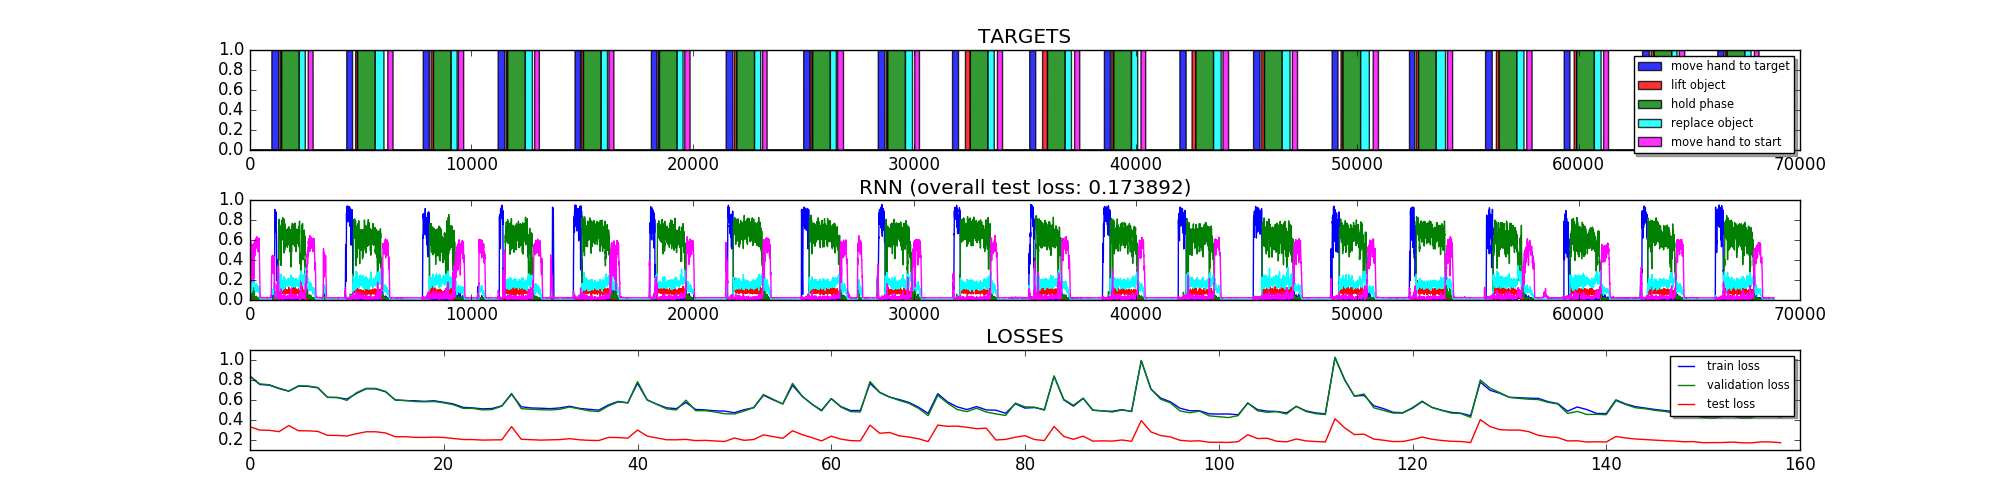
\includegraphics[width=1.0\textwidth]{images/EMG-results_participant_1_series1-6.png}
	\caption{Results of RNN trained with data of participant 1, series 1-6}
	\label{fig:emg_RNN_1}
\end{figure}

So far, all this observations are made on results of a RNN, which was trained with data of just one participant. Do demonstrate that predicting the targets with data of more than one participant works similarly fine, figure \ref{fig:emg_RNN_2} visualizes the results of a RNN trained with data of four different participants. Compared to figure \ref{fig:emg_RNN_1}, the RNN with data of more participants produces lower amplitudes. However, the structure of the predictions does not change and still fits similarly well to the target vectors.
\begin{figure}
	\centering
	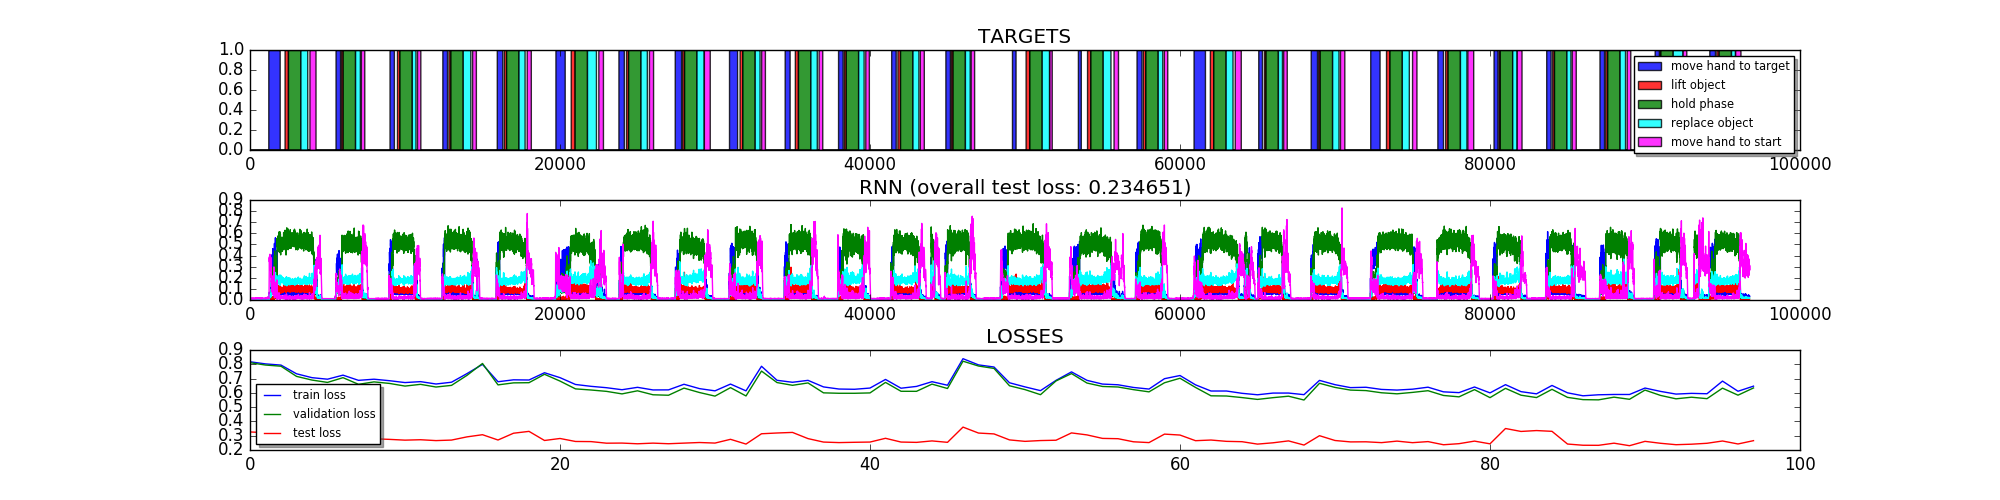
\includegraphics[width=1.0\textwidth]{images/EMG-results_participant_1-4_series1-2.png}
	\caption{Results of RNN trained with data of participant 1-4, series 1-2}
	\label{fig:emg_RNN_2}
\end{figure}

\subsection{Results using EEG-data}

\section{Summary}

\begin{thebibliography}{9}
	\bibitem{nature} 
	Luciw, M. D., Jarocka, E., Landsberger, B. B. (2014): 
	\textit{Multi-channel EEG recordings during 3,936 grasp and lift trials with varying weight and friction}. 
	 Retrieved July 20, 2016, from \\\texttt{http://www.nature.com/articles/sdata201447}.
	
	\bibitem{tsne} 
	van der Maaten, L. J. P. (2016): 
	\textit{t-SNE Implementations}.
	Retrieved July 24, 2016, from \\\texttt{http://lvdmaaten.github.io/tsne/}.
	
	\bibitem{python} 
	Python, Python Software Foundation:
	\textit{Python Language Reference, version 2.7}.
	Available at \\\texttt{http://www.python.org}
	
	\bibitem{theano} 
	Theano Development Team:
	\textit{A Python framework for fast computation of mathematical expressions by Theano Development Team}.
	Available at \\\texttt{http://arxiv.org/abs/1605.02688}.
	
	\bibitem{climin} 
	Bayer, J., Osendorfer, C., Diot-Girard, S., Rückstiess, T., Urban, S. (2016):
	\textit{climin - A pythonic framework for gradient-based function optimization}.
	 TUM Tech Report. Available at \\\texttt{http://github.com/BRML/climin}.
	 
	 \bibitem{breze} 
	 Breze.
	 Available at \\\texttt{https://github.com/breze-no-salt/breze}.
\end{thebibliography}

%\subsubsection*{References}
%[1] Luciw, M. D., Jarocka, E., EdinLandsberger, B. B. (2014) Multi-channel EEG recordings during 3,936 grasp and lift trials with varying weight and friction. Retrieved July 20, 2016, from http://www.nature.com/articles/sdata201447.

%[2] van der Maaten, L. J. P., (2016) t-SNE Implementations. Retrieved July 24, 2016, from http://lvdmaaten.github.io/tsne/.

%[3] Python, Python Software Foundation. Python Language Reference, version 2.7. Available at http://www.python.org

%[4] Theano: A Python framework for fast computation of mathematical expressions by Theano Development Team, available at http://arxiv.org/abs/1605.02688 (2016)

%@ARTICLE{2016arXiv160502688short,
%   author = {{Theano Development Team}},
%    title = "{Theano: A {Python} framework for fast computation of mathematical expressions}",
%  journal = {arXiv e-prints},
%   volume = {abs/1605.02688},
% primaryClass = "cs.SC",
% keywords = {Computer Science - Symbolic Computation, Computer Science - Learning, Computer Science - Mathematical Software},
%     year = 2016,
%    month = may,
%      url = {http://arxiv.org/abs/1605.02688},
%}

%[5] Climin: J. Bayer and C. Osendorfer and S. Diot-Girard and T. Rückstiess and Sebastian Urban. climin - A pythonic framework for gradient-based function optimization. TUM Tech Report. 2016. http://github.com/BRML/climin

%[6] Breze available at: https://github.com/breze-no-salt/breze (2016)

\end{document}
